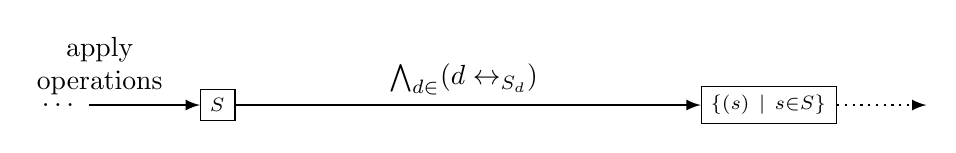
\begin{tikzpicture}[>=latex]
    %\node[draw,align=center] at (3.25, 1.75) {For all $d \in \derivedvars:$\\create BDD $S_d[\vars]$};
    \node[] at (1,0) (dots) {\dots};
    \node[draw] at (3,0) (states) {$\charf_{S}$};
    \node[draw] at (10.0,0) (fullstates) {$\charf_{\{\axioms{}(s) ~\mid~ s \in S\}}$};

    \draw[->, thick] (dots) -- (states) node[pos=0.1,above,align=center] {apply\\operations};
    \draw[->, thick] (states) -- (fullstates) node[midway,above,align=center] {$\bigwedge_{d \in \derivedvars} (d \leftrightarrow \charf_{S_d})$ };
    \draw[->,dotted,thick] (fullstates) -- (12.0,0);
\end{tikzpicture}
